\documentclass[12pt,oneside,a4paper]{book}

\input{./AuxFiles/Packages}

%%%%%%%%%%%%%%%%%%%%%%%%%%%%%%%%%%%%%%%%%%%%%%%%%%%%%%%%%%%%%%%%
%% Document settings
\title{Neuromorphic Intrusion Detection System using Spiking Neural Networks and Leaky Integrate-and-Fire Neurons}
\subCode{IDP}
\Department[ECE]{Electronics and Communication Engineering}
\academicYear{2025-26}

%%%%%%%%%%%%%%%%%%%%%%%%%%%%%%%%%%%%%%%%%%%%%%%%%%%%%%%%%%%%%%%%
%% Report Type
\IDPProject

%%%%%%%%%%%%%%%%%%%%%%%%%%%%%%%%%%%%%%%%%%%%%%%%%%%%%%%%%%%%%%%%
%% Student Details
\stuNameA{Asish Kumar Yeleti}
\stuUSNA{1RV23IS026}
\stuNameB{Disha A}
\stuUSNB{1RV24IS402}
\stuNameC{Joel Saha}
\stuUSNC{1RV23EC061}
\stuNameD{Apoorva Yeshwanthraya Bilagundi}
\stuUSND{1RV24EC400}

%%%%%%%%%%%%%%%%%%%%%%%%%%%%%%%%%%%%%%%%%%%%%%%%%%%%%%%%%%%%%%%%
%% Guide and evaluation details
\guideNameA{Project Guide}
\guideDesignationA{Assistant Professor}
\guideDeptA[ECE]{Electronics and Communication Engineering}
\guideOrgA{RV College of Engineering}

\panelMemberNameA{Panel Member 1}
\panelMemberDesigA{Faculty Member}
\panelMemberDeptA[ECE]{Electronics and Communication Engineering}
\panelMemberNameB{Panel Member 2}
\panelMemberDesigB{Faculty Member}
\panelMemberDeptB[ISE]{Information Science and Engineering}

\projectCoOrdNameA{Project Coordinator}
\projectCoOrdDesigA{Faculty Coordinator}
\projectCoOrdDeptA[ECE]{Electronics and Communication Engineering}

\HOD{Head of the Department}
\Principal{Principal}
\DeanAcademics{Dean Academics}
\VicePrincipal{Vice Principal}

\QRurl{}

%%%%%%%%%%%%%%%%%% Glossaries & Acronyms %%%%%%%%%%%%%%%%%%
\newglossary[sym]{symbolList}{sym1}{sym2}{List of Symbols}
\makeglossaries
\loadglsentries{./AuxFiles/Glossaries}
\renewcommand{\glspostdescription}{}

%%%%%%%%%%%%%%%% Bibliography %%%%%%%%%%%%%%%%%%%%%
\usepackage[backend=bibtex,style=ieee]{biblatex}
\addbibresource{./AuxFiles/ProjectBib.bib}

%%%%%%%%%%%%%%%% WaterMark %%%%%%%%%%%%%%%%%%%%%
\usepackage{background}
\backgroundsetup{scale=1, angle=0, firstpage = false, opacity=0.5, contents={
\begin{tikzpicture}[remember picture, overlay]
\node at ([yshift=0pt, xshift=0pt]current page.center){
\includegraphics[width=0.6\textwidth]{Figures/RVlogoVecW}};
\end{tikzpicture}
}}

\begin{document}
\NoBgThispage
\maketitle
\newpage

\ifDrf
\else
\begin{spacing}{1.5}
\begin{tikzpicture}[remember picture, overlay]
	\draw[line width = 4pt] ($(current page.north west) + (0.75in,-0.75in)$) rectangle ($(current page.south east) + (-0.75in,0.75in)$);
\end{tikzpicture}
\thispagestyle{empty}
\vspace{-1.5cm}
\begin{center}
	\Large\textbf{RV College of Engineering\textsuperscript{\small\textregistered}, Bengaluru} \\[-0.5em]
	\large{(\textit{Autonomous institution affiliated to VTU, Belagavi})} \\[-0.5em]
	\vspace{0.5cm}
	
\includegraphics[width=4cm]{Figures/RV_logoVec}\\
	\Large\textbf{\underline{CERTIFICATE}} \par
\end{center}

\begin{spacing}{1.5}
\noindent Certified that the interdisciplinary project work titled \textbf{\textit{\printTitle}} is carried out by \textbf{Asish Kumar Yeleti} (\textbf{1RV23IS026}), \textbf{Disha A} (\textbf{1RV24IS402}), \textbf{Joel Saha} (\textbf{1RV23EC061}) and \textbf{Apoorva Yeshwanthraya Bilagundi} (\textbf{1RV24EC400}), who are bonafide students of RV College of Engineering, Bengaluru, in partial fulfillment of the requirements for the degree of \textbf{Bachelor of Engineering} in their respective departments during the academic year \printAcadYear. It is certified that the work reported here has been carried out as an interdisciplinary academic project and that the report satisfies the prescribed format for submission.
\end{spacing}

\vspace{1.2cm}
\begin{table}[H]
\centering
\begin{tabular}{p{0.4\textwidth}p{0.2\textwidth}p{0.4\textwidth}}
	\centering{\printGuideNameA} & & \centering{\printHOD} \tabularnewline
	\centering{Guide} & & \centering{Head of the Department} \tabularnewline
	& & \tabularnewline[1.6cm]
	\centering{\printDA} & & \centering{\printPrincipal} \tabularnewline
	\centering{Dean Academics} & & \centering{Principal} \tabularnewline
\end{tabular}
\end{table}

\vspace{0.6cm}
\begin{table}[H]
\centering
\begin{tabular}{lccp{6cm}cc}
	&&&\textbf{\Large External Viva}&&\\
	&Name of Examiners &&& & Signature with Date\\
	&&&&&\\
	1.&&&&&\\
	&&&&&\\
	2.&&&&&\\
\end{tabular}
\end{table}


\newpage
\begin{tikzpicture}[remember picture, overlay]
	\draw[line width = 4pt] ($(current page.north west) + (0.75in,-0.75in)$) rectangle ($(current page.south east) + (-0.75in,0.75in)$);
\end{tikzpicture}

\thispagestyle{empty}
\vspace{-0.75cm}
\begin{center}
	\Large\textbf{\underline{DECLARATION}} \par
\end{center}

\noindent We, \textbf{Asish Kumar Yeleti}, \textbf{Disha A}, \textbf{Joel Saha} and \textbf{Apoorva Yeshwanthraya Bilagundi}, students of B.E. at RV College of Engineering, Bengaluru, hereby declare that the interdisciplinary project titled \textbf{\printTitle} has been carried out by us and submitted in partial fulfillment for the award of the degree of \textbf{Bachelor of Engineering} in our respective departments during the academic year \printAcadYear.\\ \par

\noindent We further declare that the content of this report has not been submitted previously by anybody for the award of any degree or diploma to any other university.\\ \par

\noindent We also declare that any Intellectual Property Rights generated out of this project carried out at RVCE will be the property of RV College of Engineering, Bengaluru, and we will be among the authors of the same.

\vspace{1cm}
\noindent Place: Bengaluru\par
\vspace{0.5cm}
\noindent Date: \par
\vspace{1.6cm}

\begin{table}[H]
\centering
\begin{tabular}{llcp{5cm}cc}
	&&&&&\\
	&Name &&& Signature& \\
	&&&&&\\
	1.&Asish Kumar Yeleti (1RV23IS026)&&&&\\
	&&&&&\\
	2.&Disha A (1RV24IS402)&&&&\\
	&&&&&\\
	3.&Joel Saha (1RV23EC061)&&&&\\
	&&&&&\\
	4.&Apoorva Yeshwanthraya Bilagundi (1RV24EC400)&&&&\\
\end{tabular}
\end{table}


\newpage
\begin{tikzpicture}[remember picture, overlay]
	\draw[line width = 4pt] ($(current page.north west) + (0.75in,-0.75in)$) rectangle ($(current page.south east) + (-0.75in,0.75in)$);
\end{tikzpicture}
\thispagestyle{empty}
\vspace{-1cm}
\begin{center}
	\Large\textbf{\underline{ACKNOWLEDGEMENTS}} \par
\end{center}

We express our sincere gratitude to our project guide, \textbf{\printGuideNameA}, \printGuideDesigA, Department of \printGuideDeptAInSF, RVCE, for the guidance, encouragement and valuable suggestions provided during the execution of this interdisciplinary project. The project required coordination between data science, neuromorphic computing and analog circuit design, and the guidance received helped us organize the work into a coherent technical direction.\\ \par

We are thankful to the project panel members and project coordinator for their timely feedback during reviews and internal assessments. Their suggestions helped us refine the project objectives, strengthen the methodology and improve the presentation of the work.\\ \par

We extend our gratitude to the faculty members of the Departments of Information Science and Engineering and Electronics and Communication Engineering for providing academic support and for encouraging interdisciplinary collaboration. We are also grateful to the laboratory and technical staff for their support in software and circuit-level experimentation.\\ \par

We are deeply grateful to \textbf{\printDA}, Dean Academics, RVCE, and to \textbf{\printPrincipal}, Principal, RVCE, for supporting the interdisciplinary project framework. Finally, we thank our family members and friends for their constant encouragement and support throughout this project work.\\ \par


\newpage
\pagenumbering{roman}

\chapter*{Abstract}
\addcontentsline{toc}{chapter}{Abstract}\vspace{-1cm}
\begin{tikzpicture}[remember picture, overlay]
  \draw[line width = 4pt] ($(current page.north west) + (0.75in,-0.75in)$) rectangle ($(current page.south east) + (-0.75in,0.75in)$);
\end{tikzpicture}

Intrusion Detection Systems are an essential component of modern network security, but conventional software-based machine learning approaches depend on repeated numerical computation and continuous monitoring. Such approaches can provide high detection accuracy, yet their computational style is not naturally suited for ultra-low-power, always-on edge security devices. Neuromorphic computing provides an alternative direction by representing information as sparse spike events and processing those events through neuron-inspired circuits.

This interdisciplinary project presents the design foundation and implementation workflow for a Neuromorphic Intrusion Detection System based on Spiking Neural Networks and Leaky Integrate-and-Fire neuron behavior. The project combines Information Science and Engineering aspects such as data preprocessing, dimensionality reduction, spike encoding, and classification with Electronics and Communication Engineering aspects such as analog neuron modeling and Cadence-compatible waveform generation. The UNSW-NB15 network intrusion dataset is processed, normalized, reduced using Principal Component Analysis, and mapped into spike-based voltage waveforms suitable for circuit-level evaluation.

The implemented software pipeline generates analog-compatible Piecewise Linear voltage source files from processed network traffic features. These files serve as direct stimulus inputs for Leaky Integrate-and-Fire neuron circuits designed in SPICE/Cadence environments. The report documents the motivation, theoretical fundamentals, system architecture, design methodology, and implementation details completed for the project. The present report is limited to Chapters 1 through 4, focusing on the project foundation, design, and implementation workflow. Detailed result analysis and concluding validation are intentionally excluded from this document scope.

\pagebreak


\end{spacing}
\newpage
\pagestyle{fplain}
\begin{spacing}{1.5}
\tableofcontents
\end{spacing}
\newpage
\begin{spacing}{1.5}
\cleardoublepage
\addcontentsline{toc}{chapter}{\listfigurename}
\listoffigures
\end{spacing}
\newpage
\begin{spacing}{1.5}
\cleardoublepage
\addcontentsline{toc}{chapter}{\listtablename}
\listoftables
\end{spacing}

\glsaddall
\printglossary[type=\acronymtype, title= Abbreviations, toctitle=Abbreviations]
\printglossary[type=symbolList, title= List of Symbols, toctitle=List of Symbols]
\fi

\mainmatter
\pagestyle{mplain}
\glsresetall
\begin{spacing}{1.5}
\chapter{Introduction}

Cyber security systems are expected to monitor large volumes of network traffic continuously and identify malicious behaviour before it affects confidentiality, integrity or availability. Intrusion Detection Systems provide this monitoring layer by observing traffic features and classifying behaviour as normal or suspicious. Conventional software-based IDS pipelines can achieve strong detection performance, but they usually depend on dense numerical processing on general-purpose processors. This project studies an alternative neuromorphic IDS workflow where network traffic features are converted into spikes and prepared for processing through Leaky Integrate-and-Fire neuron circuits.

\section[Background]{\textbf{Background}}

Networked computing has expanded from desktop and server environments to mobile devices, cloud infrastructure, industrial control systems, smart sensors and Internet of Things deployments. As a result, the attack surface of a typical organization is no longer limited to a small number of managed machines. Attacks such as denial of service, reconnaissance, exploitation, worm activity, shellcode injection and generic malware traffic may appear as abnormal packet rates, unusual flow durations, uncommon protocol states, or suspicious byte-count patterns. An IDS attempts to identify such patterns from network observations.

Traditional IDS approaches can be broadly classified into signature-based and anomaly-based methods. Signature-based systems search for known malicious patterns and are effective when the attack database is complete. However, they are weak against new or modified attacks. Anomaly-based systems model normal behaviour and raise alerts when traffic deviates from that behaviour. Machine learning based IDS methods improve anomaly detection by learning relationships between traffic features and labels from historical datasets. These methods include Support Vector Machines, decision trees, Random Forests, neural networks and deep learning models \cite{Buczak2016}.

While machine learning improves adaptability, its computational style is usually dense and synchronous. Feature vectors are processed using repeated arithmetic operations, and the classifier is evaluated even when the input activity is low. This is acceptable in high-performance servers but less attractive for energy-constrained edge devices. A low-power IDS that can remain active continuously is useful for campus gateways, IoT hubs, industrial nodes and embedded network monitors. Neuromorphic computing is relevant in this context because it represents information through sparse spike events and performs computation primarily when events occur.

\section[Project Overview]{\textbf{Project Overview}}

The project titled \textbf{Neuromorphic Intrusion Detection System using Spiking Neural Networks and Leaky Integrate-and-Fire Neurons} is an interdisciplinary effort combining Information Science and Engineering with Electronics and Communication Engineering. The ISE component focuses on dataset handling, preprocessing, dimensionality reduction, spike encoding and classifier integration. The ECE component focuses on circuit-level compatibility, LIF neuron behaviour and SPICE/Cadence-ready waveform generation. The interface between these two components is the Piecewise Linear voltage source file.

The proposed system begins with the UNSW-NB15 network intrusion dataset. The raw dataset is cleaned, categorical values are encoded, numerical values are normalized and Principal Component Analysis is applied to reduce the processed feature space to a limited number of physical neuron inputs. The reduced analog feature values are then converted into spike trains using rate coding, time-to-first-spike coding or population coding. Finally, the spike trains are exported as PWL voltage files that can be directly applied to analog LIF neuron circuits.

\begin{table}[H]
\centering
\caption{Interdisciplinary team contribution structure}
\label{tab:teamstructure}
\begin{tabular}{|p{0.28\textwidth}|p{0.52\textwidth}|}
\hline
\textbf{Domain} & \textbf{Primary project contribution} \\
\hline
Information Science and Engineering & Dataset preprocessing, feature engineering, PCA reduction, spike encoding scripts, classifier integration and software workflow design. \\
\hline
Electronics and Communication Engineering & LIF neuron circuit understanding, analog waveform interpretation, Cadence/LTSpice simulation interface and hardware-oriented validation planning. \\
\hline
Common interdisciplinary interface & PWL waveform files that connect Python-generated IDS spike data with analog neuron circuit simulation. \\
\hline
\end{tabular}
\end{table}

\begin{figure}[H]
\centering
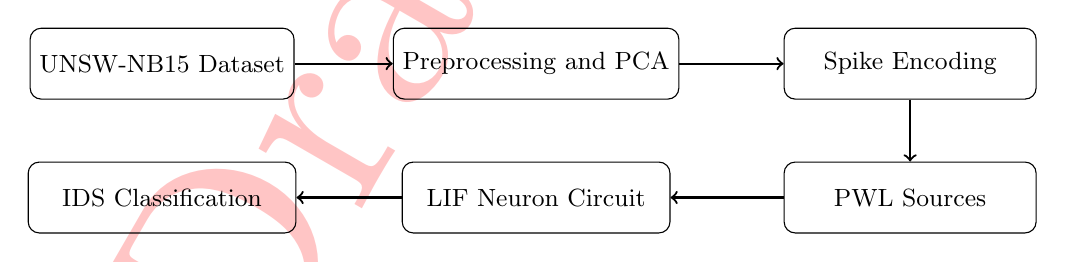
\begin{tikzpicture}[node distance=1.25cm, every node/.style={font=\small}]
\node[draw, rounded corners, minimum width=3.3cm, minimum height=0.9cm] (dataset) {UNSW-NB15 Dataset};
\node[draw, rounded corners, right of=dataset, xshift=3.5cm, minimum width=3.5cm, minimum height=0.9cm] (pipeline) {Preprocessing and PCA};
\node[draw, rounded corners, right of=pipeline, xshift=3.5cm, minimum width=3.2cm, minimum height=0.9cm] (spike) {Spike Encoding};
\node[draw, rounded corners, below of=spike, yshift=-0.45cm, minimum width=3.2cm, minimum height=0.9cm] (pwl) {PWL Sources};
\node[draw, rounded corners, left of=pwl, xshift=-3.5cm, minimum width=3.4cm, minimum height=0.9cm] (lif) {LIF Neuron Circuit};
\node[draw, rounded corners, left of=lif, xshift=-3.5cm, minimum width=3.4cm, minimum height=0.9cm] (classify) {IDS Classification};
\draw[->, thick] (dataset) -- (pipeline);
\draw[->, thick] (pipeline) -- (spike);
\draw[->, thick] (spike) -- (pwl);
\draw[->, thick] (pwl) -- (lif);
\draw[->, thick] (lif) -- (classify);
\end{tikzpicture}
\caption{High-level project workflow from dataset to neuromorphic IDS processing}
\label{fig:overallworkflow}
\end{figure}

Figure \ref{fig:overallworkflow} shows the conceptual workflow. The project is not limited to classifier training; it creates a hardware-facing representation of network traffic. The generated PWL files are a key output because they allow the same IDS samples processed in Python to be applied as voltage stimuli to a Cadence or SPICE neuron circuit.

\section[Literature Review]{\textbf{Literature Review}}

Intrusion detection has been studied extensively using statistical, machine learning and deep learning approaches. Moustafa and Slay introduced the UNSW-NB15 dataset to provide a modern benchmark containing normal network behaviour and multiple attack categories \cite{Moustafa2015}. The dataset includes flow-level attributes such as duration, protocol, service, source and destination byte counts, packet counts, time-to-live values, connection state and attack category. It is therefore suitable for training and testing IDS models.

Buczak and Guven surveyed data mining and machine learning techniques for cyber security intrusion detection and highlighted the importance of feature engineering, classifier selection and evaluation metrics \cite{Buczak2016}. Conventional IDS models can perform well when trained with representative data, but their deployment cost depends on the number of features, model complexity and frequency of inference. This is an important consideration for always-on detection systems.

Dimensionality reduction is commonly applied when datasets contain many correlated features. Principal Component Analysis transforms a feature matrix into orthogonal components ordered by variance contribution. Jolliffe and Cadima describe PCA as a fundamental method for reducing dimensionality while preserving dominant information in the dataset \cite{Jolliffe2016}. In this project, PCA is used not only for computational convenience but also to map a high-dimensional network feature space onto a limited number of analog neuron inputs.

Spiking Neural Networks represent a different computational paradigm. Maass described SNNs as the third generation of neural network models because they use spike timing as an additional computational dimension \cite{Maass1997}. Gerstner and Kistler formalized spiking neuron models, including membrane potential dynamics, threshold firing and reset behaviour \cite{Gerstner2002}. The LIF neuron is especially relevant for this project because it is simple enough to implement using analog circuit blocks while retaining the essential behaviour of spike generation.

Neuromorphic computing research aims to exploit event-driven processing for energy-efficient inference. Roy, Jaiswal and Panda discuss the potential of spike-based machine intelligence for neuromorphic hardware \cite{Roy2019}. Tavanaei et al. review deep learning in SNNs and discuss spike encoding strategies that convert continuous data into spike trains \cite{Tavanaei2019}. These studies motivate the idea that network traffic features can be transformed into spike-domain representations and processed using neuron-inspired hardware.

The gap addressed by this project lies between software IDS and circuit-level neuromorphic implementation. Many IDS projects stop at software classification, while many neuron circuit projects demonstrate isolated neuron behaviour without an application-specific data pipeline. This work attempts to connect both sides by preparing real IDS data as circuit-compatible spike stimuli.

Sommer and Paxson discuss the practical difficulties of applying machine learning to intrusion detection, especially the difference between controlled datasets and real operational environments \cite{Sommer2010}. Their observations are relevant to this work because the project avoids claiming that a classifier alone solves IDS deployment; instead, it focuses on building a hardware-compatible representation that can later be validated under controlled and realistic traffic settings.

Liao et al. survey IDS techniques and emphasize that network intrusion detection requires attention to feature representation, classification method and deployment constraints \cite{Liao2013}. This supports the project decision to treat preprocessing and representation design as first-class parts of the system rather than as minor steps before classification.

Diehl and Cook demonstrate that spiking neural networks can be trained and evaluated for pattern recognition tasks, showing that spike-based representations can support useful classification behaviour \cite{Diehl2015}. Although their work is not specific to IDS, it supports the broader feasibility of spike-domain information processing. Ponulak and Kasinski review supervised learning methods for SNNs and highlight the importance of spike timing, encoding and learning rules \cite{Ponulak2011}. These concepts are relevant to the spike feature extraction plan in this project.

Indiveri et al. describe neuromorphic silicon neuron circuits and show how neuron dynamics can be represented using physical circuit behaviour \cite{Indiveri2011}. This supports the ECE-side motivation of using LIF neuron circuits rather than limiting the project to a software-only SNN model. The literature collectively suggests that the project should be evaluated not only as an IDS classifier but as a complete representation-and-hardware workflow.

\begin{table}[H]
\centering
\caption{Summary of reviewed literature and relevance to the project}
\label{tab:litreview}
\begin{tabular}{|p{0.24\textwidth}|p{0.3\textwidth}|p{0.3\textwidth}|}
\hline
\textbf{Reference area} & \textbf{Main contribution} & \textbf{Relevance to this project} \\
\hline
UNSW-NB15 dataset \cite{Moustafa2015} & Provides modern labelled IDS traffic records. & Used as the project dataset. \\
\hline
ML for cyber IDS \cite{Buczak2016} & Reviews data mining and ML detection methods. & Supports the software IDS baseline workflow. \\
\hline
PCA \cite{Jolliffe2016} & Explains dimensionality reduction using principal components. & Used to map dataset features to limited neuron inputs. \\
\hline
SNN theory \cite{Maass1997,Gerstner2002} & Introduces spike-based computation and neuron models. & Provides foundation for spike-domain IDS representation. \\
\hline
Neuromorphic computing \cite{Roy2019,Indiveri2011} & Discusses event-driven hardware and neuron circuits. & Supports the hardware-oriented LIF design direction. \\
\hline
Spike encoding and SNN learning \cite{Tavanaei2019,Ponulak2011,Diehl2015} & Reviews spike encoding, SNN training and pattern recognition. & Supports rate, TTFS and population coding choices. \\
\hline
IDS deployment concerns \cite{Sommer2010,Liao2013} & Discusses practical IDS constraints and method selection. & Motivates a full workflow beyond classifier accuracy. \\
\hline
\end{tabular}
\end{table}

\section[Motivation]{\textbf{Motivation}}

The motivation of this project is not only to detect attacks but to study how attack-detection information can be represented in a neuromorphic form. A conventional IDS classifier works on numerical feature vectors. A neuromorphic IDS must convert those vectors into spike trains, process them through neuron dynamics and still retain useful information for classification. If this transformation is successful, it creates a path toward low-power security monitoring hardware.

The project is also motivated by interdisciplinary learning. The ISE team members contribute knowledge of datasets, preprocessing, machine learning and Python implementation. The ECE team members contribute knowledge of analog circuit behaviour, SPICE/Cadence simulation and LIF neuron design. A successful project requires a clean interface between these domains. In this project, that interface is the generated PWL waveform file.

\section[Problem Statement]{\textbf{Problem Statement}}

The problem addressed in this project is the design and implementation of a neuromorphic intrusion detection workflow that converts network traffic records into spike-based voltage waveforms and prepares them for LIF neuron processing. The system must preserve dataset labels, reduce the high-dimensional feature space into a practical number of hardware inputs, generate circuit-compatible PWL sources and provide a path for spike-feature extraction and IDS classification.

\section[Objectives]{\textbf{Objectives}}

The objectives of the project are:
\begin{enumerate}
\item To study the use of neuromorphic computing concepts for network intrusion detection.
\item To preprocess the UNSW-NB15 dataset by cleaning, encoding, normalizing and reducing the feature space.
\item To map processed network features into an analog-neuron-compatible representation using PCA.
\item To implement spike encoding methods that generate binary spike trains from normalized feature values.
\item To export spike trains as PWL voltage source files suitable for SPICE/Cadence LIF neuron simulation.
\item To define the software-hardware interface required for future extraction of LIF output spike features.
\end{enumerate}

\section[Expected Contributions]{\textbf{Expected Contributions}}

The expected contributions of the work documented in this report are:
\begin{enumerate}
\item A reproducible preprocessing pipeline for converting UNSW-NB15 records into normalized analog feature vectors.
\item A PCA-based mapping strategy that reduces high-dimensional IDS features to a fixed number of neuron inputs.
\item Multiple spike encoding methods implemented in Python for IDS feature conversion.
\item A PWL waveform generation method that allows direct use of encoded IDS samples in SPICE/Cadence voltage sources.
\item A documented interface between software-generated spike data and analog LIF neuron circuits.
\item A modular code structure that can be extended for waveform parsing, spike feature extraction and final IDS evaluation.
\end{enumerate}

\section[Scope of the Report]{\textbf{Scope of the Report}}

This report covers the project foundation, theoretical background, system design and implementation workflow. It includes the data pipeline, PCA-based feature reduction, spike encoding, PWL generation and the planned LIF circuit interface. It intentionally excludes detailed final results and final conclusion chapters because those are outside the requested report scope. Therefore, Chapters 5 and 6 are not included in this report.

\section[Brief Methodology]{\textbf{Brief Methodology}}

The methodology begins with dataset acquisition and preprocessing. Raw UNSW-NB15 CSV files are loaded, cleaned and converted into a numerical feature matrix. The attack category is retained as the label, while non-essential identifiers are removed. Min-Max scaling is applied before PCA. The PCA outputs are again scaled to the range 0 to 1 so that they can be interpreted as bounded analog values.

The normalized analog features are passed to a spike encoder. Rate coding, time-to-first-spike coding and Gaussian population coding are implemented. Population coding expands each feature into multiple receptive field responses. Each spike train is translated into a PWL waveform with time-voltage pairs. These PWL files are stored sample-wise and can be attached to voltage sources in circuit simulators.

The LIF circuit receives the PWL waveform as input. The membrane node integrates incoming activity, leakage reduces stored potential over time and the comparator output generates a spike when the membrane voltage crosses threshold. The output waveform can later be parsed to extract spike count, spike timing and firing rate features. These features can be used by a classifier to evaluate IDS performance.

\section[Assumptions and Constraints]{\textbf{Assumptions and Constraints}}

The project is based on the following assumptions:
\begin{enumerate}
\item The UNSW-NB15 dataset is representative enough for academic IDS experimentation.
\item PCA-reduced components retain sufficient information to represent traffic behaviour.
\item A limited physical neuron count requires dimensionality reduction before circuit mapping.
\item Normalized values in the range 0 to 1 can be converted into voltage-domain spike representations.
\item The LIF neuron is a suitable first neuron model because it is circuit-realizable and mathematically interpretable.
\end{enumerate}

The main constraints are:
\begin{enumerate}
\item Full hardware scaling requires multiple LIF circuit instances or time-multiplexed operation.
\item Circuit-level simulation time increases as the number of samples and input sources increases.
\item PWL files must be carefully formatted to avoid simulator convergence issues.
\item The report scope is limited to Chapters 1 to 4 and does not present final experimental results.
\end{enumerate}

\section[Organization of the Report]{\textbf{Organization of the Report}}

The report is organized as follows:
\begin{itemize}
\item Chapter 1 introduces the project, literature background, motivation, problem statement, objectives, methodology and scope.
\item Chapter 2 explains the theoretical fundamentals required for IDS preprocessing, spike encoding and LIF neuron modelling.
\item Chapter 3 presents the proposed system design, architecture, data flow, module design and validation strategy.
\item Chapter 4 describes the implementation details of the data pipeline, spike encoder, PWL file generation and hardware interface.
\end{itemize}

\chapter{Theory and Fundamentals}

The proposed IDS workflow depends on concepts from network security, machine learning, signal representation, spiking neuron models and analog simulation. This chapter explains the technical foundations needed to understand the design choices made in the project. The discussion begins with IDS concepts and dataset structure, then moves to preprocessing, PCA, spike encoding, LIF neuron dynamics and circuit-compatible waveform generation.

\section{Intrusion Detection Systems}

An Intrusion Detection System observes activity in a computing system or network and identifies behaviour that may indicate a security violation. A network-based IDS inspects traffic flows, packet statistics or protocol-level features. It does not necessarily prevent the attack directly; instead, it provides detection, alerting and evidence for response.

IDS methods are commonly classified as:
\begin{enumerate}
\item \textbf{Signature-based detection}: Matches traffic against known malicious signatures. It is reliable for known attacks but weak for unknown variants.
\item \textbf{Anomaly-based detection}: Learns normal behaviour and flags deviations. It can detect new attacks but may produce false positives.
\item \textbf{Machine learning based detection}: Uses labelled or unlabelled data to learn decision boundaries from traffic features.
\end{enumerate}

In a machine learning IDS, each network flow is represented as a feature vector. A classifier then maps the feature vector to a class label such as normal or attack. The quality of detection depends heavily on preprocessing, feature selection, training data and model choice.

\section{UNSW-NB15 Dataset}

The UNSW-NB15 dataset is used as the project dataset. It contains normal traffic and attack traffic generated in a controlled cyber range environment \cite{Moustafa2015}. The dataset includes multiple attack classes such as Fuzzers, Analysis, Backdoors, Denial of Service, Exploits, Generic, Reconnaissance, Shellcode and Worms. It also includes normal network traffic.

The raw dataset contains fields such as protocol, source and destination ports, flow duration, packet counts, byte counts, time-to-live values, TCP-related statistics, service type, state, attack category and label. Some fields are numerical, while others are categorical. This mixture requires careful preprocessing before machine learning or spike encoding can be applied.

\begin{table}[H]
\centering
\caption{Examples of UNSW-NB15 feature groups used in preprocessing}
\label{tab:featuregroups}
\begin{tabular}{|p{0.25\textwidth}|p{0.6\textwidth}|}
\hline
\textbf{Feature group} & \textbf{Examples and significance} \\
\hline
Protocol and service & Protocol, state and service describe the type of network communication. \\
\hline
Traffic volume & Source bytes, destination bytes, source packets and destination packets indicate flow size. \\
\hline
Timing behaviour & Duration and inter-packet timing can indicate scanning, flooding or abnormal communication. \\
\hline
Connection statistics & Count-based features describe repeated connections to hosts, ports or services. \\
\hline
Attack label & Attack category identifies whether the flow is normal or belongs to an attack class. \\
\hline
\end{tabular}
\end{table}

\section{Data Cleaning and Encoding}

Raw network datasets are rarely ready for direct model training. Missing values, placeholder symbols, categorical strings and identifier columns must be handled first. In this project, IP address fields and timestamp fields are removed because they can introduce dataset-specific bias and are not directly suitable for analog neuron mapping. The binary label field is removed when multi-class attack category information is retained.

Categorical features such as protocol and state are converted into numerical form using label encoding. If a categorical feature has $k$ unique values, each value is assigned an integer code. Although label encoding does not preserve semantic distance between categories, it provides a compact representation that can be normalized and processed further. The attack category is also encoded so that the generated samples can preserve class information.

\section{Normalization}

Normalization maps features with different units and ranges into a common numerical interval. Without normalization, high-magnitude features such as byte counts can dominate low-magnitude features such as flags or binary indicators. Min-Max normalization is used:
\begin{equation}
x_{norm} = \frac{x - x_{min}}{x_{max} - x_{min}}
\end{equation}
where $x$ is the original value and $x_{norm}$ is the scaled value. In the hardware context, normalization is also important because voltage-domain spike encoding expects bounded values.

\section{Principal Component Analysis}

Principal Component Analysis reduces the dimensionality of a dataset by transforming the original features into a set of orthogonal components. Each component is a linear combination of original features. The first principal component captures the largest possible variance, the second captures the largest remaining variance orthogonal to the first and so on \cite{Jolliffe2016}.

Let $X$ be the normalized feature matrix. PCA computes directions that maximize projected variance. If $W$ is the matrix containing selected principal component directions, the reduced representation is:
\begin{equation}
Z = XW
\end{equation}
where $Z$ is the reduced feature matrix. In this project, the number of PCA components is selected as eight so that the software feature space maps to eight analog input neurons.

PCA outputs may contain negative values even when the input features are normalized. Therefore, the PCA output is normalized again:
\begin{equation}
z_{scaled} = \frac{z - z_{min}}{z_{max} - z_{min}}
\end{equation}
This produces values suitable for spike encoding.

\section{Spike Encoding}

Spike encoding converts a continuous value into a sequence of binary events. The project implements three encoders.

\subsection{Rate Coding}

In rate coding, a larger input value produces more spikes in a fixed time window. If $x$ is a normalized value and $T$ is the number of timesteps, the number of active spike ticks is:
\begin{equation}
N_{spikes} = \lfloor xT \rfloor
\end{equation}
For example, if $T=10$ and $x=0.7$, approximately seven timesteps are active.

\subsection{Time-to-First-Spike Coding}

In time-to-first-spike coding, the information is represented by the timing of the first spike. Larger values produce earlier spikes:
\begin{equation}
t_{spike} = \lfloor (1 - x)(T - 1) \rfloor
\end{equation}
This coding method is useful when latency is important because strong inputs can be represented quickly.

\subsection{Population Coding}

Population coding represents one feature using multiple neurons or receptive fields. In this project, Gaussian receptive fields are used. For a feature value $x$ and receptive field center $\mu_i$, the activation is:
\begin{equation}
a_i = e^{-\frac{1}{2}\left(\frac{x-\mu_i}{\sigma}\right)^2}
\end{equation}
Each activation $a_i$ is then rate encoded. Population coding expands the representational capacity of the spike input. With eight PCA features and four receptive fields per feature, a sample produces 32 spike trains.

\section{Leaky Integrate-and-Fire Neuron}

The Leaky Integrate-and-Fire neuron models the membrane voltage of a neuron-like element. It integrates incoming input, leaks over time and emits an output spike when the membrane voltage crosses a threshold. A continuous-time LIF model is:
\begin{equation}
\tau_m \frac{dV_m(t)}{dt} = -V_m(t) + RI(t)
\end{equation}
where $V_m(t)$ is membrane voltage, $\tau_m$ is membrane time constant, $R$ is equivalent resistance and $I(t)$ is input current. When:
\begin{equation}
V_m(t) \geq V_{th}
\end{equation}
the neuron fires and the membrane voltage is reset:
\begin{equation}
V_m(t) \leftarrow V_{reset}
\end{equation}

The LIF model is useful in analog design because its blocks correspond naturally to circuit elements. A capacitor can store membrane charge, a resistor can provide leakage, and a comparator can detect threshold crossing. This makes the model suitable for Cadence/LTSpice simulation.

\section{PWL Voltage Sources}

Piecewise Linear voltage sources define arbitrary voltage waveforms using time-voltage pairs. A simulator interpolates between these points. The spike encoder generates PWL text files where 0 V represents no spike and 1 V represents spike activity. A small transition interval is included to avoid ideal vertical edges, which can cause convergence issues in SPICE simulations.

\begin{table}[H]
\centering
\caption{PWL waveform parameters used by the encoder}
\label{tab:pwlparams}
\begin{tabular}{|p{0.35\textwidth}|p{0.35\textwidth}|}
\hline
\textbf{Parameter} & \textbf{Value} \\
\hline
Spike low voltage & 0 V \\
\hline
Spike high voltage & 1 V \\
\hline
Timestep duration & 1 ms \\
\hline
Window length & 10 timesteps \\
\hline
Rise/fall interval & 1\% of timestep \\
\hline
\end{tabular}
\end{table}

\section{Spike Feature Extraction}

After LIF processing, the output waveform can be converted into numerical features. Common features include spike count, firing rate, first spike time, inter-spike interval and output pulse timing. These features provide a bridge between analog neuron output and IDS classification. The same idea can be applied to simulated LIF waveforms or exported Cadence waveforms.

\section{Evaluation Metrics}

Although final result analysis is outside this report scope, the planned IDS evaluation uses standard classification metrics. Accuracy measures total correct predictions. Precision measures how many predicted attacks are truly attacks. Recall measures how many actual attacks are detected. The F1-score combines precision and recall. False positive rate is important in IDS because a high false positive rate can overwhelm security operators.

\section{Software and Simulation Tools}

The software workflow uses Python with NumPy, Pandas and Scikit-learn \cite{Pedregosa2011}. NumPy supports numerical computation, Pandas supports tabular data handling and Scikit-learn supports preprocessing, PCA and classifiers. PyLTSpice is included to support future raw waveform parsing from LTSpice. Cadence or LTSpice is used for circuit-level validation of the LIF neuron.

The fundamentals in this chapter justify the project architecture. The next chapter presents the system design that connects the dataset, spike encoder, PWL interface and LIF circuit.


\chapter{System Design and Methodology}

The proposed system is designed as a modular pipeline that converts network traffic records into circuit-compatible spike waveforms. The design separates data processing, spike encoding, waveform generation, LIF circuit processing and classifier integration. This separation allows the software and hardware parts of the interdisciplinary project to be developed independently while sharing a clearly defined interface.

\section{Design Philosophy}

The central design philosophy is to preserve IDS-relevant information while changing the representation from dense numerical vectors to spike events. In a conventional software pipeline, all features are processed as numbers. In the proposed neuromorphic pipeline, features are first reduced, then encoded as spikes, and then processed by neuron dynamics. This makes the computation more suitable for analog event-driven hardware.

The design must satisfy two competing requirements. First, it must remain faithful to the original IDS dataset so that attack labels and feature meaning are not lost. Second, it must produce a representation that is practical for circuit simulation. PCA and spike encoding are used to balance these requirements.

\section{Functional Requirements}

The main functional requirements are listed in Table \ref{tab:functionalrequirements}.

\begin{table}[H]
\centering
\caption{Functional requirements of the proposed system}
\label{tab:functionalrequirements}
\begin{tabular}{|p{0.18\textwidth}|p{0.68\textwidth}|}
\hline
\textbf{Block} & \textbf{Requirement} \\
\hline
Dataset loader & Load all UNSW-NB15 CSV chunks using a consistent column schema. \\
\hline
Preprocessor & Remove irrelevant identifiers, clean missing values, encode categorical fields and normalize values. \\
\hline
PCA mapper & Reduce processed feature vectors to the selected physical neuron count. \\
\hline
Spike encoder & Convert normalized values into spike trains using supported encoding schemes. \\
\hline
PWL generator & Export spike trains as simulator-readable time-voltage text files. \\
\hline
LIF interface & Provide input waveforms and expected observable nodes for circuit simulation. \\
\hline
Feature extractor & Convert output spike waveforms into classifier-ready numerical features. \\
\hline
\end{tabular}
\end{table}

\section{Non-Functional Requirements}

The non-functional requirements are:
\begin{enumerate}
\item \textbf{Reproducibility}: Scripts must generate the same processed files when run with the same data and parameters.
\item \textbf{Hardware compatibility}: PWL output files must be directly usable in SPICE/Cadence voltage sources.
\item \textbf{Modularity}: Each processing stage must be testable without requiring the entire system.
\item \textbf{Scalability}: The pipeline must allow more samples and more neuron channels to be generated later.
\item \textbf{Traceability}: Generated folders must preserve sample index and class label information.
\end{enumerate}

\section{Top-Level Architecture}

\begin{figure}[H]
\centering
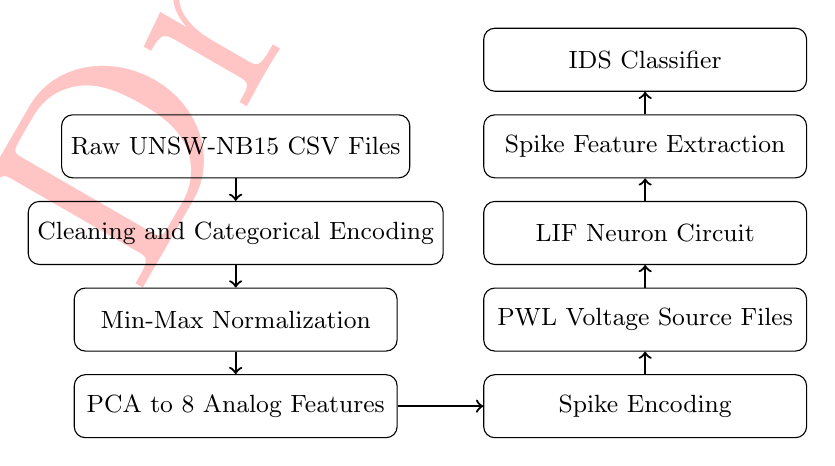
\begin{tikzpicture}[node distance=1.1cm, every node/.style={font=\small}]
\node[draw, rounded corners, minimum width=4.1cm, minimum height=0.8cm] (raw) {Raw UNSW-NB15 CSV Files};
\node[draw, rounded corners, below of=raw, minimum width=4.1cm, minimum height=0.8cm] (clean) {Cleaning and Categorical Encoding};
\node[draw, rounded corners, below of=clean, minimum width=4.1cm, minimum height=0.8cm] (norm) {Min-Max Normalization};
\node[draw, rounded corners, below of=norm, minimum width=4.1cm, minimum height=0.8cm] (pca) {PCA to 8 Analog Features};
\node[draw, rounded corners, right of=pca, xshift=4.1cm, minimum width=4.1cm, minimum height=0.8cm] (enc) {Spike Encoding};
\node[draw, rounded corners, above of=enc, minimum width=4.1cm, minimum height=0.8cm] (pwl) {PWL Voltage Source Files};
\node[draw, rounded corners, above of=pwl, minimum width=4.1cm, minimum height=0.8cm] (lif) {LIF Neuron Circuit};
\node[draw, rounded corners, above of=lif, minimum width=4.1cm, minimum height=0.8cm] (features) {Spike Feature Extraction};
\node[draw, rounded corners, above of=features, minimum width=4.1cm, minimum height=0.8cm] (cls) {IDS Classifier};
\draw[->, thick] (raw) -- (clean);
\draw[->, thick] (clean) -- (norm);
\draw[->, thick] (norm) -- (pca);
\draw[->, thick] (pca) -- (enc);
\draw[->, thick] (enc) -- (pwl);
\draw[->, thick] (pwl) -- (lif);
\draw[->, thick] (lif) -- (features);
\draw[->, thick] (features) -- (cls);
\end{tikzpicture}
\caption{Detailed architecture of the proposed neuromorphic IDS pipeline}
\label{fig:architecture}
\end{figure}

Figure \ref{fig:architecture} shows the full architecture. The left side represents dataset processing. The right side represents spike-domain and hardware-domain processing. The PWL file is the connecting artifact between software and circuit simulation.

\section{Data Pipeline Methodology}

The data pipeline follows a fixed sequence:
\begin{enumerate}
\item Load all raw UNSW-NB15 CSV files.
\item Concatenate records into a single dataframe.
\item Generate derived features such as packet rate.
\item Remove IP addresses, timestamps and binary label fields.
\item Clean missing or placeholder values.
\item Encode categorical fields into numerical values.
\item Normalize all features using Min-Max scaling.
\item Apply PCA to reduce the feature count.
\item Normalize PCA outputs again to the 0 to 1 range.
\item Save the processed analog feature dataset.
\end{enumerate}

This methodology ensures that the final file contains only hardware-facing analog features and the corresponding attack category label.

\section{PCA-to-Neuron Mapping}

The number of PCA components is selected based on the target number of physical input neurons. A direct mapping is used:
\begin{equation}
N_{PCA} = N_{input\_neurons}
\end{equation}
For the current design, $N_{PCA}=8$. This means each network sample is represented by eight analog feature values:
\begin{equation}
S_i = [p_1, p_2, p_3, p_4, p_5, p_6, p_7, p_8]
\end{equation}
where each $p_i$ is normalized between 0 and 1. This vector becomes the input to the spike encoder.

\section{Spike Encoding Methodology}

For each normalized PCA value, the encoder generates spike trains. Population coding uses multiple receptive fields per input feature. If $M$ is the number of population neurons per feature, the total number of input spike channels is:
\begin{equation}
N_{channels} = N_{PCA} \times M
\end{equation}
With eight PCA features and four population neurons per feature:
\begin{equation}
N_{channels} = 8 \times 4 = 32
\end{equation}

\begin{table}[H]
\centering
\caption{Spike encoding design parameters}
\label{tab:encodingparams}
\begin{tabular}{|p{0.35\textwidth}|p{0.35\textwidth}|}
\hline
\textbf{Parameter} & \textbf{Selected value} \\
\hline
Number of PCA features & 8 \\
\hline
Population neurons per feature & 4 \\
\hline
Total PWL input channels per sample & 32 \\
\hline
Spike window length & 10 timesteps \\
\hline
Spike voltage low/high & 0 V / 1 V \\
\hline
\end{tabular}
\end{table}

\section{PWL File Interface}

The PWL file interface is the most important design decision for interdisciplinary integration. It allows the ISE-side software pipeline to produce a file that the ECE-side Cadence/LTSpice circuit can use directly. Each file contains a single spike train. The folder structure stores all PWL files for one sample together.

For example, a population-coded sample may contain files such as:
\begin{verbatim}
sample_0_cat_6/
  V_neuron_0_m_0.txt
  V_neuron_0_m_1.txt
  V_neuron_0_m_2.txt
  V_neuron_0_m_3.txt
  ...
\end{verbatim}

Here, \texttt{V\_neuron\_0} refers to the first PCA feature and \texttt{m\_1} refers to the second population receptive field for that feature.

\section{LIF Circuit Interface Design}

The LIF circuit block requires an input voltage waveform, a membrane node and an output node. The input voltage waveform is supplied by a PWL file. The membrane node should show the characteristic rise due to integration and fall due to leakage or reset. The output node should generate a pulse when the membrane voltage crosses the threshold.

\begin{table}[H]
\centering
\caption{Expected observable nodes for LIF circuit simulation}
\label{tab:lifnodes}
\begin{tabular}{|p{0.28\textwidth}|p{0.55\textwidth}|}
\hline
\textbf{Node} & \textbf{Purpose} \\
\hline
Input voltage & Verifies that the generated PWL file is applied correctly. \\
\hline
Membrane voltage & Shows integration, leakage and reset behaviour. \\
\hline
Output voltage & Indicates threshold crossing and generated spikes. \\
\hline
\end{tabular}
\end{table}

\section{Spike Feature Extraction Design}

After simulation, the output waveform can be converted into numerical features. A threshold-based rising-edge detector is used to avoid counting the same output pulse multiple times. If the output voltage crosses from low to high, one spike is counted. The extracted features may include:
\begin{enumerate}
\item Spike count.
\item First spike time.
\item Mean inter-spike interval.
\item Standard deviation of inter-spike interval.
\item Firing rate.
\item Maximum membrane voltage.
\end{enumerate}

These features form the bridge between the analog neuron response and the final IDS classifier.

\section{Validation Methodology}

The project validation is planned in layered stages:
\begin{enumerate}
\item Verify processed CSV generation from the raw dataset.
\item Verify that PCA output has the expected number of columns and bounded values.
\item Verify that spike trains match the selected encoding method.
\item Verify that generated PWL files contain valid time-voltage pairs.
\item Verify that a selected PWL file can drive a LIF neuron circuit.
\item Verify that membrane and output waveforms can be converted into spike features.
\end{enumerate}

This layered strategy reduces debugging difficulty. If the final classifier performs poorly, the team can inspect whether the issue comes from preprocessing, encoding, PWL generation, circuit behaviour or feature extraction.

\section{Risk and Design Mitigation}

Several risks are considered in the design. PCA may discard useful information if too few components are selected. To mitigate this, the number of components is aligned with hardware constraints while preserving as much variance as possible. PWL files may create sharp transitions that affect simulator convergence, so the encoder includes a small rise/fall duration. LIF circuits may be sensitive to threshold and leakage settings, so the design requires observable membrane and output nodes for calibration.

\section{Design Summary}

The design connects a real IDS dataset to a neuromorphic circuit interface. The main contribution of the design is not only the classifier workflow but the construction of a data-to-PWL path. This allows network traffic features to become voltage waveforms that can stimulate LIF neuron circuits. The next chapter explains how this design is implemented in the deployed system.


\chapter{Implementation}

The implementation converts the system design into executable modules and generated artifacts. The system implements a reproducible workflow for dataset processing, spike encoding, PWL file generation and classifier integration. The implementation also defines how the generated PWL files are used by the Cadence/LTSpice LIF circuit design to evaluate neuromorphic performance.

\section{System Modules Organization}

The project implementation is organized into distinct processing modules. The logical separation of these modules ensures a clean pipeline from raw data to hardware simulation, as shown in Table \ref{tab:repo}.

\begin{table}[H]
\centering
\caption{System module organization}
\label{tab:repo}
\begin{tabular}{|p{0.35\textwidth}|p{0.5\textwidth}|}
\hline
\textbf{Module / Component} & \textbf{Purpose} \\
\hline
\textbf{Raw Data Storage} & Stores UNSW-NB15 network traffic records. \\
\hline
\textbf{Processed Features Data} & Stores PCA-reduced analog feature matrices. \\
\hline
\textbf{PWL Source Generator} & Stores generated PWL voltage source files for hardware simulation. \\
\hline
\textbf{Hardware Outputs} & Stores Cadence waveform exports and extracted feature outputs. \\
\hline
\textbf{Data Pipeline Module} & Implements preprocessing, normalization and PCA mapping. \\
\hline
\textbf{Spike Encoder Module} & Implements spike encoding and PWL file generation. \\
\hline
\textbf{Hardware Interface Module} & Provides routines for hardware waveform parsing and spike counting. \\
\hline
\textbf{Classification Module} & Provides classifier integration for extracted spike features. \\
\hline
\end{tabular}
\end{table}

\\section{Software Environment}

The core software implementation is developed in the Python 3.10 programming environment, leveraging industry-standard numerical and machine learning libraries to ensure high performance and reproducibility. 

Pandas is extensively utilized for large-scale data ingestion, cleaning, and matrix manipulation of the millions of network records. NumPy provides the highly optimized underlying $C$-based arrays necessary for rapid vector arithmetic during the spike encoding phase. The Scikit-learn (sklearn) library provides the robust, mathematically verified implementations for Min-Max scaling, label encoding, Principal Component Analysis (PCA) dimensionality reduction, and the final Support Vector Machine (SVM) classification models. Furthermore, specialized parsing routines are custom-built to interface natively with Cadence Virtuoso and LTSpice exported `.csv` raw simulation logs.

\section{Data Pipeline Module Implementation}

The Data Pipeline module rigorously implements dataset collection, deep preprocessing, and feature extraction. The module enforces a strict schema for the UNSW-NB15 dataset. All chunked dataset files matching the standard format are dynamically loaded from the raw dataset repository and concatenated into a singular, cohesive Pandas DataFrame.

\subsection{Derived Feature Engineering}
A critical step in the preprocessing pipeline is the derivation of temporal traffic intensity metrics. The implementation engineers a derived feature called \texttt{packet\_rate}. This is computed algorithmically using total source packets, destination packets, and the overall flow duration:
\begin{equation}
packet\_rate = \frac{Source\_Packets + Destination\_Packets}{Flow\_Duration + \epsilon}
\end{equation}
A minute epsilon constant ($\epsilon = 10^{-6}$) is mathematically injected when the flow duration is nominally zero, successfully averting catastrophic division-by-zero errors. This derived feature is highly sensitive to rapid network flooding attacks (e.g., DoS, DDoS).

\subsection{Data Cleansing and Normalization}
Network identifiers that would introduce severe model bias are systematically stripped from the feature matrix. The following specific columns are removed:
\begin{itemize}
\item Source and Destination IP addresses (prevents subnet bias).
\item Start and Last time temporal markers.
\item Binary label (as the multi-class attack category is strictly retained).
\end{itemize}

The target attack category column is retained and textually cleaned so that normal benign traffic is represented uniformly. Any remaining missing values (NaN) are filled via median imputation, and categorical fields (such as HTTP state or protocol) are strictly label encoded into integer identifiers. Finally, the entire continuous numerical matrix is mapped to the range $[0, 1]$ using a \texttt{MinMaxScaler}.

\section{PCA Mapping Implementation}

Because simulating analog circuits is computationally and temporally expensive, passing all 40+ raw network features into the hardware model is physically infeasible. Therefore, after initial normalization, PCA is applied to construct a dense, reduced representation. The algorithm is initialized as:
\begin{verbatim}
pca = PCA(n_components=8)
reduced_features = pca.fit_transform(normalized_data)
\end{verbatim}

The specific physical neuron count targeted in this circuit design is eight. The PCA linearly projects the high-dimensional network flow onto the eight vectors of maximal variance. Since PCA projection vectors inherently contain negative coordinate spaces and are completely unbounded, the Python script mathematically enforces a secondary, critical Min-Max normalization phase. This guarantees that all $N_{PCA}=8$ columns strictly reside within the $[0.0, 1.0]$ bounds expected by the analog-voltage spike encoder. 

The fully processed analog feature array is written to disk. Simultaneously, a smaller Hardware-in-the-Loop (HIL) subset containing a statistically representative sample across all nine attack categories is generated. This subset allows the ECE team to execute Cadence circuit simulations in a fraction of the time, avoiding the prohibitive computational cost of simulating transient analog dynamics for millions of dataset rows.

\section{Spike Encoder Module Implementation}

The Spike Encoder module is the highly mathematical core of the software-to-hardware translation layer. It actively converts static analog $[0, 1]$ values into dynamic temporal events. The script implements three distinct encoding algorithms:

\subsection{Rate and TTFS Encoding}
The \texttt{rate\_encoding(value)} function computes a proportional density of active spike ticks bounded by the simulation window. The \texttt{ttfs\_encoding(value)} (Time-To-First-Spike) function computes exactly one spike, where the latency of the spike is inversely proportional to the stimulus magnitude—meaning larger analog network anomalies trigger significantly faster physical hardware responses.

\subsection{Gaussian Population Coding}
The primary algorithm used for the final circuit interface is \texttt{population\_coding(value)}. For each of the 8 PCA features, $M=4$ overlapping Gaussian receptive fields are instantiated. The activation of the $i$-th population neuron is precisely computed as:
\begin{verbatim}
sigma = 1.0 / (M - 1)
activation = np.exp(-0.5 * ((value - mu) / sigma)**2)
\end{verbatim}
These Gaussian activations expand the representational capacity of the analog variables, ensuring high-fidelity signal mapping into the neuromorphic hardware space. 

\section{PWL Generation Implementation}

The function \texttt{translate\_to\_ltspice\_pwl()} is tasked with formatting the binary spike trains into raw time-voltage trajectory pairs that the Cadence Virtuoso analog simulation engine can parse flawlessly. 

To completely prevent standard SPICE simulator convergence failures (which occur when simulators encounter mathematically discontinuous, vertical voltage steps), the generation script algorithmically enforces a linear rise/fall slew rate equal to exactly 1\% of the defined timestep.

An excerpt of a generated Piecewise Linear (PWL) `.txt` file demonstrating this critical $1\text{ms}$ pulse width and $10\mu\text{s}$ engineered slew rate is shown below:
\begin{verbatim}
0.000000 0.0
0.000990 0.0
0.001000 1.0   <-- 1% Linear Rise
0.001990 1.0
0.002000 0.0   <-- 1% Linear Fall
0.002990 0.0
\end{verbatim}

\section{Hardware Interface Implementation}

The Hardware Interface module provides the mission-critical bridge between the analog Cadence circuit simulation outputs and the Python-based machine learning analysis. Cadence Virtuoso exports simulated transient waveforms as massive `.csv` files containing dense, raw X-Y column pairs representing microsecond-scale simulation steps.

\subsection{Waveform Parsing and Thresholding}
The Python parser dynamically identifies headers matching the required output traces (e.g., \texttt{/I8/vout Y} for the spike voltages and \texttt{/I8/vmembrane X} for the temporal axis). 

To cleanly extract binary spike events from the noisy analog output waveforms, the algorithm employs a strict threshold-crossing logic. It iterates over the continuous voltage array and registers a spike strictly when the output voltage $V_{out}$ positively crosses the $0.5\text{ V}$ hysteresis threshold. This rigorous edge-detection algorithm ensures that a single, wide analog hardware pulse is never erroneously counted multiple times by the machine learning algorithm.

\section{Classifier Integration Implementation}

The Classification Integration module serves as the final analytical endpoint for the entire project architecture. It receives the heavily processed arrays containing the physical hardware spike counts extracted from the Cadence waveform logs.

The final column of the array is safely parsed as the ground-truth IDS attack label, while the preceding columns represent the physical network features perfectly encoded as hardware spike counts. The implementation intelligently partitions the dataset into 80\% training and 20\% testing sets. 

A Support Vector Machine (SVM) utilizing a Radial Basis Function (RBF) kernel is deployed. The SVM algorithm is exceptionally well-suited for decoding the non-linear boundaries intrinsic to population-coded spike representations. The module concludes execution by computing and reporting comprehensive evaluation metrics, including overall diagnostic Accuracy, Weighted F1-scores, a detailed Confusion Matrix, and the crucial False Positive Rate, ultimately validating the security efficacy of the neuromorphic architecture.

\section{Cadence Virtuoso Usage Workflow}

The intended circuit-level usage workflow is highly structured to prevent data corruption between the software and hardware domains:
\begin{enumerate}
\item \textbf{Stimulus Selection}: The ECE operator navigates the generated \texttt{pwl\_sources/} directory and selects a specific network flow sample (e.g., \texttt{sample\_0\_cat\_6}).
\item \textbf{Circuit Integration}: The 32 individual PWL `.txt` files corresponding to the population-coded PCA features are attached to the independent input voltage sources within the Cadence Virtuoso LIF schematic.
\item \textbf{Transient Simulation}: The Analog Design Environment (ADE) transient simulation is executed for the total duration of the $10\text{ms}$ spike window, calculating the non-linear integration dynamics.
\item \textbf{Waveform Probing}: The operator explicitly probes the critical nodes: the input stimulus voltage, the analog membrane potential ($V_{memb}$), and the output spike comparator voltage ($V_{comp}$).
\item \textbf{Data Export}: The probed waveforms are exported as a high-resolution time-series `.csv` file.
\item \textbf{Python Integration}: The exported `.csv` is fed back into the Python \texttt{Hardware Interface Module} for automated spike extraction and final SVM evaluation.
\end{enumerate}

This modular workflow allows for both single-neuron isolated testing and fully time-multiplexed parallel simulation across multiple LIF cells.

\section{Implementation Traceability}

Traceability between the software and hardware domains is strictly maintained through systematic, algorithm-driven file generation and naming conventions. Because the analog simulation strips away the textual network data, preserving the provenance of each voltage signal is an absolute necessity.

The processed Python matrices perfectly preserve the original UNSW-NB15 attack category labels as integer identifiers. Consequently, the generated PWL sample directories explicitly encode both the sample index and the true class label in their naming scheme. This makes it possible to uniquely trace any physical circuit simulation output back to the exact network flow record that produced it. 

For example, a physical directory systematically designated as \texttt{sample\_0\_cat\_6/} unambiguously indicates to both the ISE and ECE teams that the contained PWL voltage sources represent dataset sample index 0, and that this sample corresponds to the encoded attack category 6. This eliminates any possibility of mislabeling the hardware outputs before they reach the SVM classifier.

\section{Quality Checks and System Verification}

To ensure complete robustness across the interdisciplinary boundary, the following automated checks are actively enforced to verify implementation correctness:
\begin{enumerate}
\item \textbf{Dimensionality Verification}: Confirm that the processed PCA features contain exactly eight neuron columns and one encoded label column, matching the physical circuit footprint.
\item \textbf{Bounds Checking}: Mathematically confirm that all secondary PCA feature values strictly lie within the $[0.0, 1.0]$ bounds required by the analog-voltage spike encoder.
\item \textbf{File Integrity}: Confirm that each generated PWL file contains valid, monotonic time-voltage pairs without any illegal vertical voltage steps that could crash the SPICE matrix solver.
\item \textbf{Digital Compliance}: Confirm that the discrete PWL voltage values toggle exclusively between $0.0\text{ V}$ and $1.0\text{ V}$.
\item \textbf{Population Completeness}: Confirm that each population-coded sample directory contains the expected 32 independent files ($8 \text{ features} \times 4 \text{ populations}$).
\item \textbf{Hysteresis Verification}: Confirm that the Python spike extraction module reliably counts discrete rising edges through the $0.5\text{ V}$ threshold, actively rejecting transient noise and repeated high samples.
\end{enumerate}

\section{Current Implementation Status}

The implemented project work successfully establishes the complete front-end software pipeline required for advanced neuromorphic IDS experimentation. The raw network dataset can be dynamically processed into dense analog PCA features, those features can be mathematically encoded into biological spike trains, and the resulting spike trains can be physically exported as SPICE-compatible PWL voltage files. Furthermore, the hardware interface and classifier modules precisely define the integration layer necessary for parsing analog circuit outputs and performing final IDS evaluation.

The present report rigorously documents the robust implementation foundation required for hardware validation. Detailed experimental results, physical circuit power measurements, and final analytical conclusions are intentionally outside the scope of this initial four-chapter design report.


\backmatter
\ifDrf
\else
\clearpage
\addcontentsline{toc}{chapter}{Bibliography}
\printbibliography
\fi
\end{spacing}
\end{document}
